\PassOptionsToPackage{unicode=true}{hyperref} % options for packages loaded elsewhere
\PassOptionsToPackage{hyphens}{url}
%
\documentclass[english,,man]{apa6}
\usepackage{lmodern}
\usepackage{amssymb,amsmath}
\usepackage{ifxetex,ifluatex}
\usepackage{fixltx2e} % provides \textsubscript
\ifnum 0\ifxetex 1\fi\ifluatex 1\fi=0 % if pdftex
  \usepackage[T1]{fontenc}
  \usepackage[utf8]{inputenc}
  \usepackage{textcomp} % provides euro and other symbols
\else % if luatex or xelatex
  \usepackage{unicode-math}
  \defaultfontfeatures{Ligatures=TeX,Scale=MatchLowercase}
\fi
% use upquote if available, for straight quotes in verbatim environments
\IfFileExists{upquote.sty}{\usepackage{upquote}}{}
% use microtype if available
\IfFileExists{microtype.sty}{%
\usepackage[]{microtype}
\UseMicrotypeSet[protrusion]{basicmath} % disable protrusion for tt fonts
}{}
\IfFileExists{parskip.sty}{%
\usepackage{parskip}
}{% else
\setlength{\parindent}{0pt}
\setlength{\parskip}{6pt plus 2pt minus 1pt}
}
\usepackage{hyperref}
\hypersetup{
            pdftitle={Does Every Study? Implementing Ordinal Constraint in Meta-Analysis},
            pdfauthor={Julia M. Haaf1 \& Jeffrey N. Rouder2},
            pdfkeywords={keywords},
            pdfborder={0 0 0},
            breaklinks=true}
\urlstyle{same}  % don't use monospace font for urls
\usepackage{graphicx,grffile}
\makeatletter
\def\maxwidth{\ifdim\Gin@nat@width>\linewidth\linewidth\else\Gin@nat@width\fi}
\def\maxheight{\ifdim\Gin@nat@height>\textheight\textheight\else\Gin@nat@height\fi}
\makeatother
% Scale images if necessary, so that they will not overflow the page
% margins by default, and it is still possible to overwrite the defaults
% using explicit options in \includegraphics[width, height, ...]{}
\setkeys{Gin}{width=\maxwidth,height=\maxheight,keepaspectratio}
\setlength{\emergencystretch}{3em}  % prevent overfull lines
\providecommand{\tightlist}{%
  \setlength{\itemsep}{0pt}\setlength{\parskip}{0pt}}
\setcounter{secnumdepth}{0}

% set default figure placement to htbp
\makeatletter
\def\fps@figure{htbp}
\makeatother

% Manuscript styling
\usepackage{upgreek}
\captionsetup{font=singlespacing,justification=justified}

% Table formatting
\usepackage{longtable}
\usepackage{lscape}
% \usepackage[counterclockwise]{rotating}   % Landscape page setup for large tables
\usepackage{multirow}		% Table styling
\usepackage{tabularx}		% Control Column width
\usepackage[flushleft]{threeparttable}	% Allows for three part tables with a specified notes section
\usepackage{threeparttablex}            % Lets threeparttable work with longtable

% Create new environments so endfloat can handle them
% \newenvironment{ltable}
%   {\begin{landscape}\begin{center}\begin{threeparttable}}
%   {\end{threeparttable}\end{center}\end{landscape}}
\newenvironment{lltable}{\begin{landscape}\begin{center}\begin{ThreePartTable}}{\end{ThreePartTable}\end{center}\end{landscape}}

% Enables adjusting longtable caption width to table width
% Solution found at http://golatex.de/longtable-mit-caption-so-breit-wie-die-tabelle-t15767.html
\makeatletter
\newcommand\LastLTentrywidth{1em}
\newlength\longtablewidth
\setlength{\longtablewidth}{1in}
\newcommand{\getlongtablewidth}{\begingroup \ifcsname LT@\roman{LT@tables}\endcsname \global\longtablewidth=0pt \renewcommand{\LT@entry}[2]{\global\advance\longtablewidth by ##2\relax\gdef\LastLTentrywidth{##2}}\@nameuse{LT@\roman{LT@tables}} \fi \endgroup}

% \setlength{\parindent}{0.5in}
% \setlength{\parskip}{0pt plus 0pt minus 0pt}

% \usepackage{etoolbox}
\makeatletter
\patchcmd{\HyOrg@maketitle}
  {\section{\normalfont\normalsize\abstractname}}
  {\section*{\normalfont\normalsize\abstractname}}
  {}{\typeout{Failed to patch abstract.}}
\patchcmd{\HyOrg@maketitle}
  {\section{\protect\normalfont{\@title}}}
  {\section*{\protect\normalfont{\@title}}}
  {}{\typeout{Failed to patch title.}}
\makeatother
\shorttitle{Ordinal Constraint in Meta-Analysis}
\keywords{keywords\newline\indent Word count: X}
\DeclareDelayedFloatFlavor{ThreePartTable}{table}
\DeclareDelayedFloatFlavor{lltable}{table}
\DeclareDelayedFloatFlavor*{longtable}{table}
\makeatletter
\renewcommand{\efloat@iwrite}[1]{\immediate\expandafter\protected@write\csname efloat@post#1\endcsname{}}
\makeatother
\usepackage{csquotes}
\usepackage{mathrsfs}
\usepackage[makeroom]{cancel}
\usepackage{pcl}
\usepackage{setspace}\doublespacing
\usepackage{marginnote}
\newcommand{\readme}[1]{\emph{\marginnote{Julia} (#1)}}
\usepackage{pifont}
\ifnum 0\ifxetex 1\fi\ifluatex 1\fi=0 % if pdftex
  \usepackage[shorthands=off,main=english]{babel}
\else
  % load polyglossia as late as possible as it *could* call bidi if RTL lang (e.g. Hebrew or Arabic)
  \usepackage{polyglossia}
  \setmainlanguage[]{english}
\fi

\title{Does Every Study? Implementing Ordinal Constraint in Meta-Analysis}
\author{Julia M. Haaf\textsuperscript{1} \& Jeffrey N. Rouder\textsuperscript{2}}
\date{}


\authornote{

Julia M. Haaf, Psychological Methods Unit, University of Amsterdam, Amsterdam, Netherlands; Jeffrey N. Rouder, Department of Cognitive Sciences, University of California, Irvine, USA.

We are indebted to Sho Tsuji and Julia Carbajal for letting us use their familiar-word-recognition meta-analysis and for helping us make sense of the interpretation of the findings. We thank Paul Speckman and Quentin Gronau for insightful discussions about variable transformations and meta-analysis. This manuscript and analysis code are available at XXX.

Correspondence concerning this article should be addressed to Julia M. Haaf, Postbus 15906, 1001 NK AMSTERDAM, The Netherlands. E-mail: \href{mailto:j.m.haaf@uva.nl}{\nolinkurl{j.m.haaf@uva.nl}}

}

\affiliation{\vspace{0.5cm}\textsuperscript{1} University of Amsterdam\\\textsuperscript{2} University of California-Irvine}

\abstract{
The most prominent goal when conducting a meta-analysis is to estimate the true effect size across a set of studies. This approach is problematic whenever the analyzed studies are inconsistent, i.e.~some studies show an effect in the predicted direction while others show no effect and still others show an effect in the opposite direction. In case of such an inconsistency, the average effect may be a product of a mixture of mechanisms. The first question in any meta-analysis should therefore be whether all studies show an effect in the same direction. To tackle this question a model with multiple ordinal constraints is proposed - one constraint for each study in the set. This ``every study'' model is compared to a set of alternative models, such as an unconstrained model that predicts effects in both directions. If the ordinal constraints hold, one underlying mechanism may suffice to explain the results from all studies. A major implication is then that average effects become interpretable. We illustrate the model-comparison approach using Carbajal et al.'s (2020) meta-analysis on the familiar-word-recognition effect, show how predictor analyses can be incorporated in the approach, and provide R-code for interested researchers. As common in meta-analysis, only surface statistics (such as effect size and sample size) are provided from each study, and the modeling approach can be adapted to suit these conditions.
}



\begin{document}
\maketitle

The common goals in meta-analysis are to measure a meta-analytic mean, and to assess how this mean depends on covariates. For example, we may want to know whether infants can distinguish familiar words from novel words (Carbajal, Peperkamp, \& Tsuji, 2020). The common method to study infant word recognition is to present familiar and novel words, and to measure the difference in either looking times or head turns. Because the data are relatively expensive in infant research, meta-analysis is an important tool to gain more precision. Using meta-analysis, the overall familiar-word-recognition effect can be assessed across a set of studies, and the variable age, for example, could serve as a covariate for theoretical development and guidance of future studies.

Although targeting meta-analytic means may seem uncontroversial, we have previously argued alternative targets are more appropriate (Rouder, Haaf, Davis-Stober, \& Hilgard, 2019). We started with the observation that for many experimental paradigms positive, zero, and negative effects correspond to different psychological phenomena. For the familiar-word-recognition effect these three domains - negative, null, positive - correspond to different stages in early language development (Hallé \& Boysson-Bardies, 1994). During the first few months babies do not distinguish familiar words and rare or novel words, and studies investigating the familiar-word-recognition effect with up to 11 month old infants may expect a zero effect. During the next stage of language development, infants may pay more attention to familiar words than novel ones resulting in an expected positive familiar-word-recognition effect. After around 20 months processing of words changes again, and infants may even pay more attention to novel words (Hallé \& Boysson-Bardies, 1994). This distinction between negative, zero, and positive effects poses a problem for conventional meta-analysis. Imagine you had an effect size of 0.4 in one study, and of -0.2 in another. How well does the average of 0.1 describe the two studies? Can we conclude that there is a small positive familiar-word-recognition effect where babies pay more attention to familiar words than novel words?

Motivated by the concern that qualitatively different outcomes correspond to different psychological processes Rouder et al. (2019) recommend assessing whether all true study effects are in the same qualitative region. The distinction between true and observed effects is critical here. A true effect is a study's underlying latent effect, and if the study had infinitely many trials and participants we could observe its true effect. In reality though, we only observe a limited number of trials and participants, and this limited knowledge introduces sample noise. The observed effect is therefore a combination of the true effect and sample noise. Sample noise increases the variability of a collection of observed effects in that observed effects are more variable than true effects. To separate sample noise and true variability Rouder et al. (2019) used hierarchical modeling. This tool allows to take sample noise into account, and to answer questions about the collection of true effects.

If all true effects are plausibly in the same direction the average across these effects is much more interpretable as an overall effect of common phenomenology. Conversely, if true effects are in opposite directions, the average in uninterpretable. This issue is discussed in the clinical literature as \emph{quantitative} vs.~\emph{qualitative interactions} (Gail \& Simon, 1985; Pan \& Wolfe, 1997). In a clinical setting, qualitative interaction refers to the case that one treatment is superior for one patient population, and another treatment is superior for another patient population. In this case, recommendation for treatment has to be qualified by the target population. Gail and Simon (1985) propose testing for qualitative interactions in meta-analysis, and Higgins, Thompson, and Spiegelhalter (2009) discuss Bayesian estimation-based methods for such a test. We call testing for qualitative interactions a \emph{does-every-study meta-analysis}.

One of the main contributions of Rouder et al. (2019) is a Bayesian model-comparison method of determining whether a set of studies plausibly share a common phenomenology. There are three obvious constrained models to consider: A \emph{positive-effects model} where all true study effects are constrained to be positive, a \emph{negative-effects model} where all true study effects are constrained to be negative, and a \emph{null model} where all study effects are constrained to be exactly zero. The alternative to these constrained models is a mixture where some studies are negative, positive, and null. Rouder et al. (2019) called this mixture the \emph{unconstrained model}. Knowing whether the unconstrained model holds or whether one of the constrained models hold is critical for understanding any psychological phenomenon, and to determine the required theoretical complexity. The four models will be developed subsequently.

The approach by Rouder et al. (2019) is based on the development by Haaf and Rouder (2017) for Bayesian model comparison, and the required inputs for the hierarchical models assessed are the raw, participant-level data from each study. There are four concerns with this approach when applied to meta-analysis: First, while there are some examples of collections of studies where raw data are available (e.g.~Ebersole et al., 2016; Corker, Donnellan, Kim, Schwartz, \& Zamboanga, 2017; Wagenmakers et al., 2016), the vast majority of meta-analyses is based on published summary statistics rather than raw data. Second, in many meta-analyses the dependent measures and designs vary across studies. For example, dependent variables may be accuracy in some studies, and response times in others. Third, the development in Rouder et al. (2019) is best suited for experimental settings and not for correlational designs. Fourth, one of the major goals of meta-analysis, assessing the effect of study-level predictor variables, was not yet addressed. In sum, the model comparison approaches that we previously advocated were simply not developed for common meta-analyses where designs and scales vary, and where data extraction relies on published information. To increase the applicability of the does-every-study meta-analysis, here we describe models for the effect size measure Fisher's \(Z\) because Fisher's \(Z\) can be calculated from extant summary statistics. The current development should be widely applicable.

In the next section, we present the collection of formal does-every-study models that we subsequently compare. Following that, we develop meta-regression approaches to understand whether covariates affect the underlying phenomenology. We apply the does-every-study analysis to meta-analytic data on the familiar-word-recognition effect reported by Carbajal et al. (2020). We discuss the importance of prior settings for Bayesian meta-analysis, limitations of the methods, and future directions of does-every-study modeling.

\hypertarget{does-every-study-models}{%
\section{Does-Every-Study Models}\label{does-every-study-models}}

First, we need to specify what are considered the data for the does-every-study models. This choice is limited by the information available in published articles. We decided to use the effect-size estimate Fisher's \(Z\) which is typically used to assess the size of a correlation coefficient. The measure is a variance stabilizing transformation of the bivariate correlation coefficient \(r\) that maps \(r\) onto the real number space. The formula for Fisher's \(Z\) is

\begin{align}\label{eq:Zcalc}
Z = \frac{1}{2} \, \ln\Big(\frac{1 + r}{1 - r}\Big) = \mbox{arctanh}(r),
\end{align}

and the asymptotic distribution of \(Z\) is a normal distribution:

\begin{align}\label{eq:fishersZ}
Z \sim \mbox{Normal}(\theta, \frac{1}{N - 3}),
\end{align}

where \(\theta\) is the true effect size and \(N\) is the number of observations. Importantly, the size of the correlation does not affect the variance of \(Z\); the variance is only dependent on \(N\). This property makes Fisher's \(Z\) an attractive target for the modeling approach. In the Appendix, we provide a proof showing that this beneficial property of Fisher's \(Z\) also holds for biserial correlations, and the modeling approach is therefore equally suitable for experimental settings with condition as the predictor.

To learn about the sign and variability of effects models are placed on the collection of study effects much like in what is often called random-effects meta-analysis. For the following models, let \(i\) denote the study, \(i = 1, \ldots, I\). The base model here is

\begin{equation}\label{eq:basemodel}
Z_i \sim \mbox{Normal}\Big(\theta_i, \frac{1}{N_i - 3}\Big),
\end{equation}

where \(\theta_i\) is the \(i\)th study's true \(Z\)-value. We may place models with ordinal and equality constraints on the collection of these true study effects \(\theta_i\).

\hypertarget{the-unconstrained-model}{%
\subsubsection{The Unconstrained Model}\label{the-unconstrained-model}}

The unconstrained model is a standard linear model without constraints, and it corresponds to the typical random-effects meta-analytic model. Here, the collection of study effects simply follows a normal distribution:

\[
\begin{array}{llr}
{\cal M}_u: && \theta_i \stackrel{iid}{\sim} \mbox{Normal}(\mu,\tau^2),\\
\end{array}
\]

where \(\mu\) is the mean effect and \(\tau^2\) is the variance of effects. No constraints are placed on the collection of \(\theta_i\) such that effects for some studies may truly be positive while effects for other studies may truly be negative.

\hypertarget{the-positive-effects-model}{%
\subsubsection{The Positive-Effects Model}\label{the-positive-effects-model}}

The positive-effects model corresponds to the hypothesis that every study has a true effect in the same, expected direction:

\[
\begin{array}{llr}
{\cal M}_p: && \theta_i \stackrel{iid}{\sim} \mbox{Normal}^+(\mu,\tau^2),\\
\end{array}
\]

where \(\mbox{Normal}^+\) is a normal distribution truncated below at zero. The positive domain of the model translates to the idea that effects are coded so that positive is the expected direction. This model statement implies multiple ordinal constraints, one for each study in the data set, reducing model complexity drastically compared to the unconstrained model. Assuming the same mean and variance as the general model, the positive-effects model has higher density for (small) positive effects and no mass below zero.

\hypertarget{the-common-effect-model}{%
\subsubsection{The Common-Effect Model}\label{the-common-effect-model}}

The common-effect model corresponds to the frequentist fixed-effect meta-analytic model (Borenstein, Hedges, Higgins, \& Rothstein, 2010). For the common-effect model, all \(\theta_i\) have the same value:

\[
  \begin{array}{llr}
{\cal M}_c: && \theta_i = \mu, \mu > 0.\\
\end{array}
\]

Here, the common effect, \(\mu\), is restricted to be in the expected direction, just like in the positive-effects model.

The common-effect model may seem unlikely, and there has been much philosophical and statistical debate about the usefulness of meta-analytic common-effect models (e.g.~Hedges \& Vevea, 1998). Surely, there must be some variability between true effects across studies. Yet, especially in meta-analysis, this model may be a necessary addition to the set of models proposed. Borenstein et al. (2010) note, for example, that between study variability may be hard to estimate with small numbers of studies in a data set. Also, the common effect assumption may be meaningful when the experiments where pre-planned to use the exact same methods across labs. This pre-planning is common in medical research, and it recently gained attention in psychological research with the many-labs projects (Ebersole et al., 2016). In fact, Rouder et al. (2019) report evidence for this model for Ebersole and colleagues' many-labs study on moral credentialism.

\hypertarget{the-null-model}{%
\subsubsection{The Null Model}\label{the-null-model}}

The last model proposed is a null model. Here, all \(\theta_i\) are exactly zero:

\[
  \begin{array}{llr}
{\cal M}_0: && \theta_i = 0.\\
\end{array}
\]

This model is the most constrained model of the set, and it is a strict null in that it does not allow for true variability around zero. Instead, all variation must be captured in the noise term \(\frac{1}{N_i - 3}\). If an effect truly does not exist, then all studies truly should have a null result. True variation around zero would imply that there has to be a trade-off between the studies such that all true effects sum to zero, which is highly unlikely and violates the independence assumption of the data. \emph{\marginnote{Julia} (Did we say this anywhere?)}

\hypertarget{prior-settings}{%
\subsubsection{Prior Settings}\label{prior-settings}}

For Bayesian analysis, priors are needed on the mean and variance parameters. Here, prior distributions are placed on \(\mu\), the true mean effect size, and on \(\tau^2\), the true variability of effect sizes. We chose conjugate prior distributions:

\begin{align*}
\mu &\sim \mbox{Normal}(0, 0.15^2),\\
\tau^2 &\sim \mbox{Inverse-Gamma}(1, 0.02).
\end{align*}

The priors on \(\mu\) and \(\tau^2\) are critical for model comparison because they differ between the models. For example, the common-effect model constrains \(\tau^2\) to zero. Therefore, the prior settings have to be chosen with care. Typically, these settings should be made by researchers familiar with the scaling of the dependent variable (Haaf \& Rouder, 2017; Rouder, Haaf, \& Aust, 2018). Here, the random variable is effect size, and one might think the scaling is obvious. Yet, we note here that different measures of effect size have different scaling, and an intuition for expected ranges of, say Cohen's \(d\) may not be helpful when developing models for Fisher's \(Z\). We believe that the current settings are appropriate for many applications in psychology. Nevertheless, a sensitivity analysis for varying prior settings is crucial to assess whether the variability of Bayes factor model comparison results are reasonable. We provide more discussion on the issue and a sensitivity analysis subsequently.

\hypertarget{model-comparison}{%
\section{Model Comparison}\label{model-comparison}}

The main purpose of the modeling approach is to draw inference about the distribution of study effects.
To do so, we propose a Bayes factor model comparison approach to compare the unconstrained model, the positive-effects model, the common-effect model, and the null model. Here, we provide an informal discussion of Bayes factors, and we briefly present the approaches used to estimate Bayes factors between the models. A more extensive discussion may be found in Jeffreys (1961), Kass and Raftery (1995), Morey, Romeijn, and Rouder (2016), and Rouder, Morey, and Wagenmakers (2016).

In Bayesian model comparison, the main target of interest is the relative evidence for one model compared to another. The Bayes factor is this relative evidence, and it results directly from Bayes rule. Bayes rule for two models, \({\cal M}_1\) and \({\cal M}_2\) is

\begin{equation}\label{bayesrule}
\frac{P({\cal M}_1 \mid \bm Y)}{P({\cal M}_2 \mid \bm Y)} = \frac{P(\bm Y\mid {\cal M}_1)}{P(\bm Y\mid {\cal M}_2)} \times \frac{P({\cal M}_1)}{P({\cal M}_2)},
\end{equation}

where \(\frac{P({\cal M}_1 \mid \bm Y)}{P({\cal M}_2 \mid \bm Y)}\) are the posterior odds, \(\frac{P({\cal M}_1)}{P({\cal M}_2)}\) are the prior odds, and \(\frac{P(\bm Y\mid {\cal M}_1)}{P(\bm Y\mid {\cal M}_2)}\) is the Bayes factor. The Bayes factor is also referred to as the updating factor because it is the amount by which the prior odds need to be updated in the light of the data to get to the posterior odds.

\begin{figure}
\centering
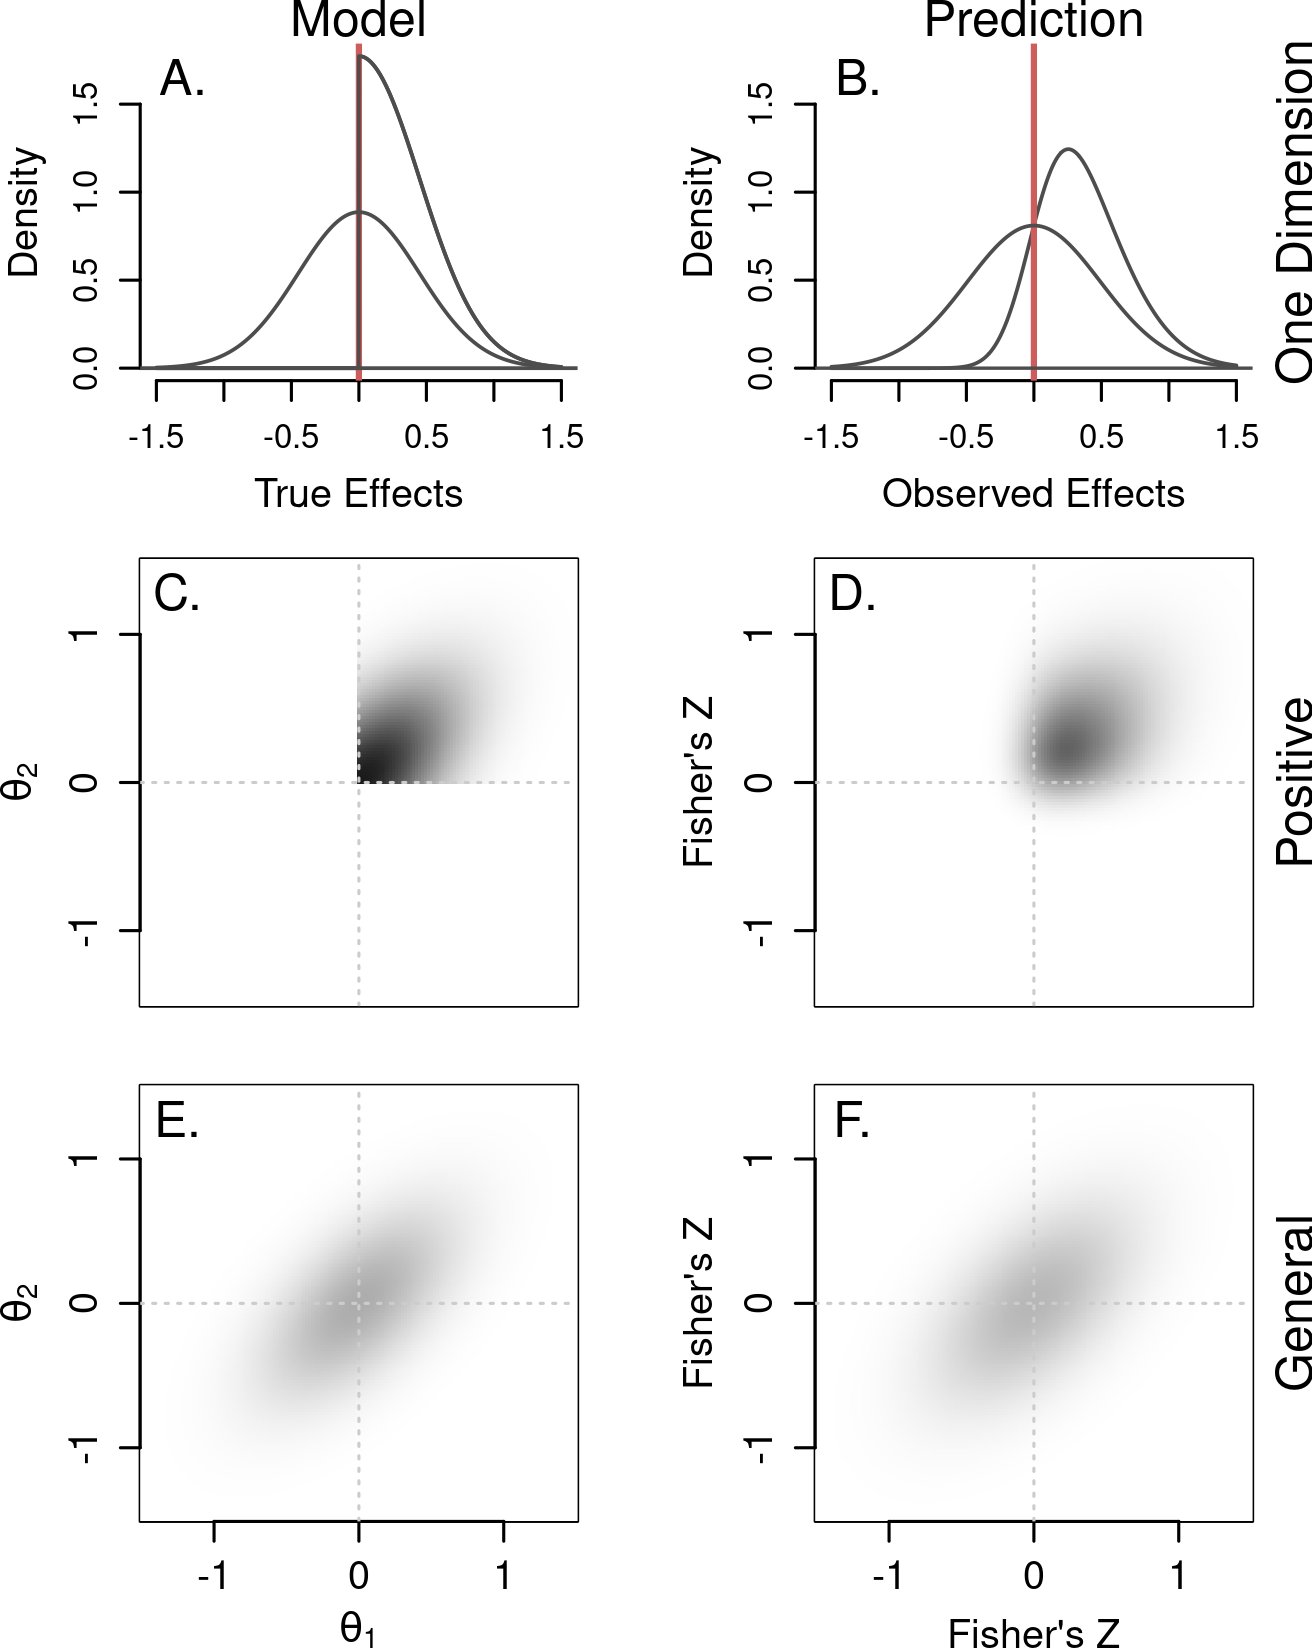
\includegraphics{p_files/figure-latex/meta-modelcomp-1.png}
\caption{\label{fig:meta-modelcomp}Model specification and predictions for the positive-effects model and the general model. The models are on the left hand-side, and the predictions for data are on the right hand-side. Top row: Models for one study. Even though the positive-effects model is restricted to positive values in specification, it can predict small negative observed values. Middle row: Positive-effects model for two studies. Effects for any two studies are predicted to be correlated due to the hiearchical nature of the model, and mostly positive. Bottom row: General model for two studies. Effects are still correlated, but may be positive or negative. The predictions for any specific effect combination is weaker for the general model as is covers more parameter space.}
\end{figure}

We may also view the Bayes factor as \emph{predictive accuracy} of Model \({\cal M}_1\) relative to the predictive accuracy of Model \({\cal M}_2\). In this sense, the Bayes factor denotes how well \({\cal M}_1\) predicted the observed data compared to \({\cal M}_2\). Figure~\ref{fig:meta-modelcomp} illustrates this point. Panel A shows the model specifications for the positive-effects and the unconstrained model for any one study's true effect. The predictions for observed effect sizes from these models are illustrated in panel B. As can be seen, the positive-effects model best predicts positive effects while the general model predicts both positive and negative effects to the same degree. As a result, if a positive effect is observed, the positive-effects model will be preferred as it has more density for positive effects than the general model. In contrast, if a negative effect is observed the general model will be preferred. Yet, the positive-effects model \emph{can} predict small negative effects despite the ordinal constraint on true effects. As a side note, it is a major advantage of Bayesian analysis to allow for the calculation of predictions from a model \emph{before} observing any data. In the frequentist setting, predictions are always based on observed data, for example using cross-validation (Rouder et al., 2016).

How do the model predictions extend to more than one study effect? Figure~\ref{fig:meta-modelcomp} shows multivariate model specifications for two studies for both the unconstrained and the positive-effects model. Panels C and D show model specification and model prediction for the positive-effects model. The effect size for Study 1 is specified on the x-axis; the effect size for Study 2 is specified on the y-axis. The correlation between the two effects is introduced by the hierarchical nature of the models (i.e.~the common variability of the mean effect), and it is a desirable feature of hierarchical modeling. This correlation is also preserved in the predictions, and the positive-effects model best predicts small, similar, positive effects. The predictions of the unconstrained model are shown in Figure~\ref{fig:meta-modelcomp}F. The model predictions again cover more of the parameter space than the predictions of the positive-effects model leading to relatively less predictive accuracy for observed positive effects.

Conceptually, Bayes factors can be understood as a comparison between the prediction in panels D anf F in Figure~\ref{fig:meta-modelcomp}. If we observed effects for the two studies, say \(z_1 = .2\) and \(z_2 = .25\), then we may compare the predictive accuracy for the point \([.2, .25]\) of the two bottom-right graphs. The ratio of the predictive accuracies at the observed data point is the Bayes factor between the two models.

Practically, Bayes factors can be estimated in several ways. Here, we use the encompassing approach to estimate the Bayes factor between the unconstrained model and the positive-effects model (Haaf \& Rouder, 2017; Hoijtink, 2012; Klugkist, Laudy, \& Hoijtink, 2005), and an analytic approach to assess the Bayes factor between the unconstrained model, the common-effect model, and the null model (Rouder, Morey, Speckman, \& Province, 2012). The Bayes factors between the positive-effects model, the common-effect model, and the null model can be obtained using the transitivity property of Bayes factors.\footnote{Using transitivity, the Bayes factor between the positive-effects model and the null model, \(B_{+0}\), may be obtained as \(B_{+0} = \frac{B_{g0}}{B_{g+}}\).}

The encompassing approach (Hoijtink, 2012) may be used to estimate Bayes factors between nested models, where one model is an order-constrained version of an encompassing model. This is the case for the unconstrained and positive-effects models. The Bayes factor is

\[
B_{u+} = \frac{P(\bm \theta> \bf0 | {\cal M}_u)}{P(\bm \theta> \bf0 | \bm Y, {\cal M}_u)},
\]

where \(\bm \theta\) is an \(I\)-dimensional vector containing \(\theta_i\), and \(\bm Y\) are the observed data. The numerator of the right-hand-side denotes the probability that all \(\theta_i\) are positive before seeing the data under the unconstrained model, and the denominator denotes the same quanitity for the posterior of the unconstrained model. Using the encompassing approach, the Bayes factor can be estimated using samples from the posterior and prior distributions of the unconstrained model \({\cal M}_u\). Using MCMC-estimation, we may sample \(M\) samples from the prior and posterior distributions of \(\theta_i\) with \(m\) indicating sample, \(m = 1, \ldots, M\). The \(m\)th sample is evidential of the positive-effects model if all \(\theta_i\) are positive. Let \(n_{0+}\) indicate the frequency of evidential samples from the prior, and let \(n_{1+}\) indicate the frequency of evidential samples from the posterior. Then, the Bayes factor between the general and the positive-effects models is approximately

\[
B_{u+} \approx \frac{n_{0+}}{n_{1+}}.
\]

The analytic approach employed here is based on Rouder et al. (2012). The main targets of the approach are the probability of data conditional on the two models marginalized over the parameter space. This probability is typically called the marginal probability of a model, and it may be expressed using The Law of Total Probability as
\begin{equation} \label{eq:bfInt}
P(\bm Y\mid {\cal M}) = \int_{\bm \xi\in \Xi} P(\bm Y|\bm \xi)P(\bm \xi)d\bm \xi,
\end{equation}
where \(\bm \xi\) is a vector of parameters from parameter space \(\Xi\). The likelihood function, \(P(\bm Y|\bm \xi)\), is given by Equation~\eqref{eq:basemodel}, and it is the product of normal densities with mean \(\theta_i\) and variance \(\frac{1}{n_i - 3}\) evaluated for the data.

Here, we illustrate the analytic approach for obtaining the Bayes factor between the null model and the unconstrained model. For the null model, obtaining the marginal probability is straight-forward. The parameter space of \(\theta_i\) is reduced to a point, to zero. The integral in Equation \eqref{eq:bfInt} is simply the likelihood of the data when \(\theta_i = 0\) for all \(i\). For the unconstrained model, the integral in Equation \eqref{eq:bfInt} may be simplified by integrating out the collection of \(\theta_i\) and the overall effect \(\mu\). The likelihood of \(Z_i\) marginal over \(\theta_i\) and \(\mu\) is

\[Z_i | \tau^2, \sigma^2_\mu \sim \mbox{Normal}(0, \frac{1}{n_i - 3} + \tau^2 + \sigma^2_\mu),\]

where \(\tau^2\) is the variance of \(\theta_i\) and \(\sigma^2_\mu\), the variance of \(\mu\) that is here fixed at \(.15^2\). The integral is now reduced to one dimension. To estimate \(P(\bm Y\mid {\cal M})\) the integral can be evaluated for possible values of \(\tau^2\) based on its prior distribution. The marginal probability can be estimated in similar fashion for the common-effect model.

\hypertarget{application-the-familiar-word-recognition-effect}{%
\section{Application: The Familiar-word-recognition Effect}\label{application-the-familiar-word-recognition-effect}}

\begin{figure}
\centering
\includegraphics{p_files/figure-latex/resFig-1.pdf}
\caption{\label{fig:resFig}Results for the familiar-word-recognition effect from the unconstrained model. Observed effects with 95\% confidence intervals are depicted by the gray squares and bars, posterior estimates with 95\% credible intervals are given by the black points and bars. There is hierarchical shrinkage to the overall effect reducing the variability of study effects drastically.}
\end{figure}

We are now ready to apply the does-everyone meta-analysis to data. Here, we re-analyzed the meta-analysis on the familiar-word-recognition-effect conducted by Carbajal et al. (2020). The authors gathered 34 studies from 0 research articles studying infants with average sample age ranging from 5 to 15 months. Here, null, positive, and negative effects correspond to different stages in early language development (Hallé \& Boysson-Bardies, 1994). If infants do not distinguish between familiar and unfamiliar words then the familiar-word-recognition effect is zero. If infants pay more attention to familiar words than novel ones then the familiar-word-recognition effect is positive. If infants pay more attention to novel words than familiar words then the familiar-word-recognition effect is negative. The expectation is that infants in the age range of the current studies show a positive familiar-word recognition effect. The analysis by Carbajal et al. (2020) showed an overall effect size in line with this expectation, \(\hat{\mu} = 0.21\), \(95\%\)CI \(= [0.13, 0.3]\).

We first estimated the unconstrained model. The observed and estimated study effect sizes (Fisher's \(Z\)) are shown in Figure~\ref{fig:resFig}. The gray squares correspond to the observed effect sizes, and the black points correspond to the estimates from the unconstrained model (posterior means). The gray error bars show the 95\% confidence intervals for Fisher's \(Z\). The black error bars show 95\% credible intervals. The size of the points is determined by the study weights that are in turn dependent on the sample size. These weightsdetermine the impact of each study on the overall effect size. As can be seen, there is a substantial amount of hierarchical shrinkage reducing the variability of estimated study effects as compared to observed study effects. The amount of shrinkage for each study is a function of the standard error of the effect size estimate, which in turn is a function of the sample size. Because the studies in the current meta-analysis have relatively small sample sizes---between 12 and 53 participants---as is typical for developmental research, hierarchical shrinkage is expected to substantially pull more extreme values towards the overall effect.

Figure~\ref{fig:resFig} also shows that while three studies have an observed negative effect size the estimates for all 34 studies are positive. To quantify the evidence for or against every-study-does, we compare the models previously proposed using Bayes factors. The preferred model is the positive-effects model, and it is preferred over the common-effect model by 3.02 to 1, over the null model by 9.43 to 1, and over the unconstrained model by 14.66 to 1. Hence, while there is some evidence that all studies show a positive effect, there is only limited evidence that study effects actually differ.

In summary, it seems that all studies conform with the expectation that infants pay more attention to novel words, but there is only limited evidence for variability of study effects across studies. On of the reasons for the lack of variability is that sample sizes are relatively small in almost all studies. Therefore, each study effect is estimated with a lot of uncertainty, and the common-effect model cannot be ruled out. However, both positive-effects and common-effect models allow for the direct interpretation of the overall effect across studies, estimated as \(\hat{\mu} \mid \bm Z= 0.20\), \(95\%\)CrI \(= [0.12, 0.29]\). This estimate can be used to inform the design of future studies. Another goal of meta-analyses, however, is to confirm the effect of predictor variables on the effect size in question. Subsequently, we will show how such predictors can be incorporated in the does-every-study approach.

\hypertarget{accounting-for-predictors}{%
\section{Accounting for Predictors}\label{accounting-for-predictors}}

A key goal in meta-analysis is to assess the relationship between a predictor variable and the effect size across studies (Borenstein, Hedges, Higgins, \& Rothstein, 2011). This is especially relevant if there is substantial between-study variability. Then, researchers might ask whether there are covariates that explain some of this between-study variability. Typically, included covariates are on the study level, for example, the experimental design or the specific choice of dependent variable. The covariate or predictor variable can either be categorical or continuous.

Here, we consider two cases that are potentially relevant for the question whether every study shows an effect in the same direction. First, we consider meta-regression models and ask whether there are qualitative interactions where studies show opposite effects, and whether there is a covariate that explains the flip. Questions related to the meta-regression approach are: After taking a covariate into account, are all effects positive? If all studies show an effect in the same direction, are all effects in the same direction even when taking a covariate into account? Second, we might ask whether studies on one level of a categorical covariate show an effect in the expected direction while studies on another level of the covariate show no effect. We call this the some-do-some-don't approach. In this section, we propose meta-regression models and a some-do-some-don't model, show how evidence for or against the effect of a predictor can be assessed, and illustrate the approach, where appropriate, by applying these models to the familiar-word-recognition meta-analysis.

\hypertarget{meta-regression}{%
\subsection{Meta-regression}\label{meta-regression}}

We start with extending the base model in Equation~\eqref{eq:basemodel} to include a covariate:

\begin{equation} \label{eq:pred}
Z_i \sim \mbox{Normal}(\theta_i + x_i \beta, \frac{1}{N_i - 3}),
\end{equation}

where \(x_i\) denotes the covariate for the \(i\)th study, and \(\beta\) denotes the slope. The covariate can be either continuous, and in this case \(x_i\) is standardized, or it can be categorical, and in this case \(x_i\) is effect-coded.

For the familiar-word-recognition meta-analysis, we may want to assess the effect of the average age of study samples on the effect size. To do so, we z-standardized age and estimated the model using gibbs sampling. Figure~\ref{fig:resfig-cont}A shows the resulting estimates and regression line. Observed effects are shrunken towards the regression line. The slope of the estimated regression line is \(\beta = 0.06\), 95\%CI \(= [-0.03, 0.14]\). Note that this slope is slightly reduced from the least square error regression line (dashed line). This reduction is due to hierarchical shrinkage of study effect sizes.

\begin{figure}
\centering
\includegraphics{p_files/figure-latex/resfig-cont-1.pdf}
\caption{\label{fig:resfig-cont}Comparison of the meta-regression and the intercept-only analysis of age. The x-axes show the standardized average age per study, the y-axes show Fisher's Z effect size estimates. Gray open points are observed effect sizes; blue points are estimated effect sizes from the Bayesian models. A. Results for the meta-regression model. The dashed line corresponds to a simple least squares regression line; the blue line corresponds to the estimated regression line from the Bayesian meta-regression model. B. Results for the intercept-only model. The dashed line corresponds to the average observed effect size; the blue line corresponds to the estimated mean from the Bayesian meta-regression model.}
\end{figure}

\hypertarget{the-positive-intercepts-approach}{%
\subsubsection{The Positive-intercepts Approach}\label{the-positive-intercepts-approach}}

The typical procedure to test the effect of a covariate in meta-analysis is to compare a regression model that includes the predictor with a model without that predictor. However, when combining regression models with the does-every-study approach, we impose additional restrictions on parameters. The positive-intercepts approach may be used if there is evidence that some studies show an opposite-to-expected effect. In this case, we want to assess whether the covariate is responsible for the opposing effects. Therefore, after taking \(\beta\) into account, we want to know whether \(\theta_i\) the study intercepts, are positive. The restriction imposed is similar to the positive-effects model:

\[
  \begin{array}{llr}
{\cal M}_{+|\beta}: && \theta_i > 0.\\
\end{array}
\]

The comparison most relevant here is therefore between the unconstrained model without predictor and the positive-intercepts model with predictor. For the familiar-word-recognition meta-analysis, we decided not to assess this model comparison because there is no evidence for qualitative study differences.

\hypertarget{the-positive-covariate-approach}{%
\subsubsection{The Positive-covariate Approach}\label{the-positive-covariate-approach}}

Even if there are no opposing study effect sizes as is the case for the familiar-word-recognition meta-analysis, we may still want to assess the effect of a covariate. In this case, the covariate nevertheless may explain some of the variability that otherwise contributes to noise variability. The effect of explained variance is evident in the comparison of Figures~\ref{fig:resfig-cont}A and B. The estimated effects from the unconstrained base model are much less variable than the estimated effects from the unconstrained meta-regression model. Therefore, it is plausible that the positive-effects model is preferred if no covariate is included because all effect sizes are estimated to be positive, but if a covariate is included some of these effect sizes may become negative. Therefore, we may want to test whether \emph{true effect sizes plausibly are positive even after taking a covariate into account.} To do so, we impose the following constraint:

\[
  \begin{array}{llr}
{\cal M}_{+\hat{z}}: && \theta_i + x_i \beta > 0.\\
\end{array}
\]

The constraint is posed on the predicted effect size, \(\hat{Z}_i\), which combines the study intercept and slope. The constraint implies that the predictor does not affect the qualitative nature of the study effect sizes. We call this model the positive-prediction model.

For the familiar-word-recognition meta-analysis, we computed Bayes factors to compare all previous models without covariate, and added the unconstrained model with covariate and the positive-prediction model. All comparisons are shown in Table~\ref{tab:covariate-tab}. The preferred model remains the positive-effects model without predictor. The unconstrained model with covariate performs poorest with a Bayes factor of 54.76-to-one in favor of the positive-effects model. The positive-prediction model, on the other hand, is the second-best model out of the bunch with a Bayes factor of 2.01-to-one in favor of the positive-effects model. The reason for the discrepancy between the positive-prediction model and the unconstrained model with covariate is the predictive accuracy---the prior probability that all predicted effect sizes given the moderator are positive is fairly low. The positive-prediction model therefore receives a boost in predictive accuracy as compared to the unconstrained model with moderator. Nevertheless, because the effect of age is so small the positive-effects model without moderator is still preferred.

\begin{table}[tbp]

\begin{center}
\begin{threeparttable}

\caption{\label{tab:covariate-tab}Bayes factors for the familiar-word-recognition meta-analysis.}

\begin{tabular}{ll}
\toprule
Model & \multicolumn{1}{c}{Bayes factor}\\
\midrule
Unconstrained Model & 1\\
Null Model & 1.55\\
Common-effect Model & 4.86\\
Positive-effects Model & 14.66\\
Unconstrained Model with Covariate & 0.27\\
Positive-prediction Model & 7.3\\
\bottomrule
\addlinespace
\end{tabular}

\begin{tablenotes}[para]
\normalsize{\textit{Note.} Bayes factors are in comparison to the unconstrained model.}
\end{tablenotes}

\end{threeparttable}
\end{center}

\end{table}

\hypertarget{some-studies-do-some-dont-approach}{%
\subsection{Some-studies-do-some-don't Approach}\label{some-studies-do-some-dont-approach}}

For this approach we ask whether a categorical variable predicts whether a study has a positive effect, or whether a study has no effect. For example, we may want to assess the effect of preregistration on effect size, and, based on the consideration of publication bias, predict that studies from registered reports show no effect while unregistered studies show an effect in the predicted direction. We refer to this setup as a \emph{some-studies} model.

\begin{figure}
\centering
\includegraphics{p_files/figure-latex/figModerator-1.pdf}
\caption{\label{fig:figModerator}Estimates for the covariate model with study type as some-studies covariate. The black points show estimated study effects from the model where some studies have a zero effect as predicted by the moderator (familiar-word-recognition effect as baseline) and some studies have positive effects as predicted by the moderator (familiar-word-recognition effect as main target of interest). For two studies (Bywater, 2004) the moderator was not reported.}
\end{figure}

With the base model from Equation~\eqref{eq:basemodel} the some-studies model can be placed on \(\theta_i\):

\[
\begin{array}{llr}
{\cal M}_{ss}: && \begin{cases}
\theta_i \stackrel{iid}{\sim} \mbox{Normal}^+(\mu,\tau^2) \quad \mbox{if} \; x_i = 1,\\
\theta_i = 0 \quad \quad \quad \quad \quad \quad \quad \; \mbox{if} \; x_i = 0.
\end{cases}
\end{array}
\]

where \(x_i\) is an dummy variable indicating whether the covariate predicts an effect (\(x_i = 1\)) or no effect (\(x_i = 0\)). Note that this model is quite constrained: Not only does it predict the direction of the effect for some studies, it also predicts zero-effects for other studies, and it \emph{a priori} assigns each study to either of the two categories. Therefore, if study effects show a pattern similar to the predicted (i.e.~the covariate predicts considerable increase of effect sizes) the predictive accuracy of the model is high.

In the meta-analysis on familiar-word-recognition the covariate of study use could be considered as a some-studies predictor. In correspondence with the authors (Carbajal et al., 2020) they mentioned the suspicion that whether the familiar-word-recognition effect was the main target of interest, or whether it was a baseline effect greatly impacted the size of the effect. They hypothesized that, because data collection in developmental psychology is costly, the data were published no matter the size of the effect if it was the target of interest. Conversely, if the effect was considered a baseline it would perhaps be omitted in case of a null finding. As a result, the familiar-word-recognition effect would be greatly inflated for studies where it was considered a baseline effect.

\begin{table}[tbp]

\begin{center}
\begin{threeparttable}

\caption{\label{tab:ss-tab}Bayes factors for the target vs. baseline study analysis.}

\begin{tabular}{ll}
\toprule
Model & \multicolumn{1}{c}{Bayes factor}\\
\midrule
Unconstrained Model & 1\\
Null Model & 2.12\\
Common-effect Model & 5.18\\
Positive-effects Model & 12.85\\
Some-studies Model & 121.16\\
\bottomrule
\addlinespace
\end{tabular}

\begin{tablenotes}[para]
\normalsize{\textit{Note.} Bayes factors are in comparison to the unconstrained model.}
\end{tablenotes}

\end{threeparttable}
\end{center}

\end{table}

We applied the some-studies model to the covariate of study use, and assigned \(x_i = 1\) to baseline studies and \(x_i = 0\) to main studies. Figure~\ref{fig:figModerator} shows estimates from the model for 32 of the 34 studies, only including the ones where the covariate was available. The majority of the studies with small effects are in the category that has the familiar-word-recognition effect as main target, and more of the studies with larger effect sizes belong to the 12 studies that reported the familiar-word-recognition effect as baseline. We compared the some-studies model with the models from the previous sections using Bayes factors (See Table~\ref{tab:ss-tab}).\^{}\{The Bayes factors for the models shown both in Table 1 and Table~\ref{tab:ss-tab} deviate slightly because less studies are included for Table~\ref{tab:ss-tab}.\} The some-studies model outperforms all the other models, and it is preferred to the positive-effects model by 9.43 to 1.

\hypertarget{software}{%
\section{Software}\label{software}}

The analyses presented here are conducted in \texttt{R} (R Core Team, 2016).\footnote{The following packages were used: R (Version 4.0.2; R Core Team, 2016) and the R-packages \emph{fields} (Version 10.3; Douglas Nychka, Reinhard Furrer, John Paige, \& Stephan Sain, 2017), \emph{ggplot2} (Version 3.3.2; Wickham, 2016), \emph{knitr} (Version 1.29; Xie, 2015), \emph{maps} (Version 3.3.0; Richard A. Becker, Ray Brownrigg. Enhancements by Thomas P Minka, \& Deckmyn., 2018), \emph{Matrix} (Version 1.2.18; Bates \& Maechler, 2018), \emph{MCMCpack} (Version 1.4.8; Martin, Quinn, \& Park, 2011), \emph{metafor} (Version 2.4.0; Viechtbauer, 2010), \emph{msm} (Version 1.6.8; Jackson, 2011), \emph{papaja} (Version 0.1.0.9997; Aust \& Barth, 2017), and \emph{psych} (Version 1.9.12.31; Revelle, 2018).} We provide an \texttt{R}-script containing all necessary functions to compute posterior estimates and Bayes factors at XXX. Functions \texttt{mcmc\_unconstrained()}, \texttt{mcmc\_moderator()}, and \texttt{mcmc\_somesstudies()} are gibbs samplers providing posterior estimates for the overall analysis and moderator analyses. Functions \texttt{get.bfs.ss()} and \texttt{get.bfs.cont()} provide Bayes factor estimation for all proposed models. The analysis of the familiar-word-recognition effect (Carbajal et al., 2020) is provided at XXX. We hope these functions help interested researchers to conduct the proposed analyses themselves.

\hypertarget{prior-sensitivity}{%
\section{Prior Sensitivity}\label{prior-sensitivity}}

Bayes factor model comparison requires the choice of prior distributions. Some prior settings have minimal influence on the results of the analysis while others have substantial influence. In the current meta-analysis the prior settings with substantial influence on inference are the priors on the variance of study effect size parameters, \(\tau^2\), and the prior setting on the variance of the overall effect size, \(\mu\). Here, we highlight how prior settings need to be adjusted based on the effect size measure used, and we show how variation of prior settings on these two parameters affects inference.

\begin{figure}
\centering
\includegraphics{p_files/figure-latex/transplot-1.pdf}
\caption{\label{fig:transplot}Effect size measures for simulated data from 100 studies with 100 participants. The panels show transformations from Cohen's d to A. Cohen's d, B. Hedges' g, C. Fisher's Z, and D. log odds ratio. While order and sign of the effect size measures are consistent the scales differ substantially.}
\end{figure}

For the current analysis we decided to use Fisher's \(Z\) as effect size measure for its beneficial properties in modeling. Fisher's \(Z\) is popular for correlational analyses, and it can be interpreted as a standardized correlation coefficient. Other effect size measures that are frequently used in psychology are Cohen's \(d\) (or its close relative Hedges' \(g\)) and log odds ratios. To quickly assess the effect of different choices of effect size measures, we simulated data from 100 experiments with 100 participants each, and calculated four different effect size measures for the same data. Figure~\ref{fig:transplot} compares Cohen's \(d\) to Hedges' \(g\), Fisher's \(Z\), and log odds ratio for the same data. As apparent from the figure, the key property for our analysis, the direction of the effect, is preserved across all transformations. However, the values of the effect size are different across measures. As a rule of thumb, Cohen's \(d\) and Hedges' \(g\) have about the same values, the value of Fisher's \(Z\) is about half of Cohen's \(d\) for the same data, and the value of log odds ratio is approximately double of Cohen's \(d\) for the same data.

This scaling difference between effect size measures does not have implications for frequentist meta-analysis as long as the measures have full support and are asymptotically normally distributed. For Bayesian meta-analysis, however, the different scaling has a substantial effect on prior specification. When using the same prior distribution on effect size for Cohen's \(d\) and Fisher's \(Z\), for example, model comparison results would differ even if the same data are used. Therefore, it is impossible to recommend default prior settings for Bayesian meta-analysis that can be applied across different effect size measures. Adjustments are needed for the variance of \(\theta_i\), \(\tau^2\), and for the variance of \(\mu\). For \(\tau^2\) we chose an inverse-gamma distribution with shape of 1 and scale of 0.02. The variance of \(\mu\) is set to \(0.15^2\). If Cohen's \(d\) is used instead of Fisher's \(Z\), a quick fix would be to double the scale on \(\tau^2\) (resulting in a scale of 0.04), and to double the standard deviation of \(\mu\) (resulting in a variance of \(0.30^2\)).

\begin{table}[tbp]

\begin{center}
\begin{threeparttable}

\caption{\label{tab:tabsens}Prior sensitivity analysis.}

\begin{tabular}{llllll}
\toprule
Shape of $\tau^2$ & \multicolumn{1}{c}{Scale of $\tau^2$} & \multicolumn{1}{c}{Variance of $\mu$} & \multicolumn{1}{c}{$BF_{pu}$} & \multicolumn{1}{c}{$BF_{pc}$} & \multicolumn{1}{c}{$BF_{p0}$}\\
\midrule
1 & 0.02 & $0.15^2$ & 14.66 & 3.02 & 9.43\\
1 & 0.04 & $0.3^2$ & 5.13 & 0.37 & 0.08\\
1 & 0.01 & $0.3^2$ & 3.91 & 0.88 & 0.19\\
1 & 0.04 & $0.08^2$ & 193.21 & 41.18 & 114.13\\
1 & 0.01 & $0.08^2$ & 32.69 & 14.32 & 39.68\\
\bottomrule
\end{tabular}

\end{threeparttable}
\end{center}

\end{table}

But how are the analyses affected by these choices? One way of assessing the influence of the choice of priors is to conduct a sensitivity analyses. In a sensitivity analysis, the variability of Bayes factors based on reasonable adjustments of prior settings is assessed (e.g., Haaf \& Rouder, 2017; Heycke, Gehrmann, Haaf, \& Stahl, 2018). Here, we conducted a sensitivity analysis for the familiar-word-recognition effect where we assessed the effect of reasonable prior settings on the Bayes factors. We chose to double and halve the scale on \(\tau^2\) from our original setting between 0.01 and 0.04), and to double and halve the standard deviation of \(\mu\) (between 0.08 and 0.30).

Table~\ref{tab:tabsens} shows the Bayes factors for the original analysis and four additional analyses varying these settings. Bayes factors are between the positive-effects model and the model in the respective column. In general, when variance and scale parameters were decreased (corresponding to smaller expected effect sizes) Bayes factors in favor of the positive-effects model compared to all other models increased (up to \(BF_{pu} = 193.21\)). When variance and scale parameters where increased (corresponding to larger expected effect sizes) Bayes factors the null model was preferred over the positive-effects model (up to \(BF_{0p} = 12.21\)). The prior on the variance of \(\mu\) seemingly has the biggest impact for the current analysis.

The results from the sensitivity analysis highlight the importance of good prior choices. Dependent on the priors, we may gain evidence for or against the effect in the current analysis. The impact of these choice, however, depends on the application, the number of studies, and the size of the target effects. To aid the interpretation of the range of prior settings used here, a scale of Fisher's \(Z\) of 0.15 corresponds to a scale on Cohen's \(d\) of \(0.30\), or a small to medium effect. If the scale on this effect size is cut in half the prior settings correspond to a predicted effect size of \(0.16\) on the Cohen's \(d\) scale. In that case there is overwhelming evidence from the data for such a small effect. Likewise, if the scale is doubled the prior settings correspond to a a predicted effect size of \(0.61\) on the Cohen's \(d\) scale, which is a sizable effect. In that case the data are more in line with the absence of an effect. Therefore, the scale settings have to reflect the expected effect size for the effect size measure that is analyzed.

\hypertarget{discussion}{%
\section{Discussion}\label{discussion}}

Meta-analysis is a powerful tool to summarize evidence across several studies. In the absence of open data it is the most straight-forward method to combine quantitative results across multiple studies. Here, we highlight a fundamental, theoretical issue with meta-analysis---the issue whether we even ask the right scientific question. Rather than solely focusing on an overall effect size, we ask whether every study in the data set shows an effect in the expected direction. This scientific question is in line with the concept of qualitative interactions (Gail \& Simon, 1985) where different treatments may be appropriate for different populations in a clinical setting. And it is also in line with considerations of replicability. In light of psychological theory, we are oftentimes more interested in the direction of an effect rather than its size (Haaf, Klaassen, \& Rouder, 2019).

To answer the question whether every study shows an effect in the same direction we develop a set of models: A general model much like the conventional meta-analytic random-effects model; a positive-effects model where all studies have an effect in the same direction; a common-effect model much like the conventional meta-analytic fixed-effect model; and a null model. To assess the relative strength of evidence between these models, we propose a Bayes factor model comparison approach adapted from Haaf and Rouder (2017) and Rouder et al. (2019). Critically, the new approach models the collection of studies' effect size measures and therefore can be applied if only surface statistics are available.

A second scientific question for meta-analysis concerns predictor variables. Oftentimes, we ask whether task or population characteristics affect the observed effect size in question. We show how the approach can be extended to include potential moderators. We apply the does-every-study meta-analysis to the familiar-word-recognition effect (Carbajal et al., 2020) in babies. In developmental research, small sample sizes are common, and meta-analysis therefore remains a central methodological approach. The results from our analysis provide evidence for the claim that studies either show a positive effect, or no effect whatsoever. We did not find a qualitative interaction where some studies show an opposite effect.

\hypertarget{limitations-and-future-directions}{%
\subsection{Limitations and Future Directions}\label{limitations-and-future-directions}}

A main limitation of the current approach is that it does not allow for the identification and correction of publication bias. Publication bias and questionable research practices are intimately tied to the question of the usefulness of meta-analysis (Carter, Schönbrodt, Hilgard, \& Gervais, 2017; Corker, 2018). If the studies in the meta-analytic set are heavily biased, using them to learn about the population is difficult. A number of correction methods for publication bias have been proposed (Duval \& Tweedie, 2000; Hedges, 1984; Iyengar \& Greenhouse, 1988; Simonsohn, Nelson, \& Simmons, 2014; Stanley \& Doucouliagos, 2014). One possible extension of the current modeling approach is to add publication bias correction measures such as selection modeling approaches (Iyengar \& Greenhouse, 1988; Maier, Bartoš, \& Wagenmakers, 2020). In principle, this extension should not be too difficult. Yet, assessing the success of these corrections can be problematic, as neither the process of study censorship nor the amount of publication bias are known in any real meta-analytic set (Guan \& Vandekerckhove, 2016; Haaf, n.d.). There is an additional problem with adding publication bias correction to the current modeling approach. To illustrate the problem, consider Figure~\ref{fig:meta-modelcomp}A. If all studies indeed have a true positive effect, then the resulting distribution of observed effects should be similar to the slightly skewed, mostly positive distribution. However, the distribution that is assumed by most publication bias correction methods is the one resulting from the general model, which is symmetric, normal-shaped. Most, if not all correction methods use a skewed distribution as an indicator for publication bias. While it may be possible to disentangle publication bias and true positive effects by assessing the relationship of sample size and effect size, auch a solution remains an open issue.

One main contribution of the current analysis compared to the analysis proposed by Rouder et al. (2019) is modeling surface statistics instead of raw data. This approach is necessary when raw study data are not available. Whenever raw data are available, we recommend using hierarchical model approaches instead of surface statistics models. Hierarchical models are better equipped to optimally model within-study variability. As open science gains more and more traction, however, it may be possible that raw data are available for some newer studies but not others. To optimally incorporate information from raw data and surface data, a hybrid modeling approach integrating the models proposed by Rouder et al. (2019) and our current analysis might be useful.

In summary, the current approach allows to investigate questions of ordinal constraint in a meta-analytic setting. We think that answering the does-every-study question is important. If, indeed, every study shows a true effect in the same, expected direction, maintaining an underlying theory for the target phenomenon seems reasonable. If, however, the ordinal constraint is violated and some studies indeed show true opposite effects, researchers need to investigate the underlying mechanism that lead to this qualitative interaction. These mechanisms may be found in design or population, and the proposed predictor analysis can help understanding the underlying differences.

\newpage

\hypertarget{references}{%
\section{References}\label{references}}

\begingroup
\setlength{\parindent}{-0.5in}
\setlength{\leftskip}{0.5in}

\hypertarget{refs}{}
\leavevmode\hypertarget{ref-R-papaja}{}%
Aust, F., \& Barth, M. (2017). \emph{papaja: Create APA manuscripts with R Markdown}. Retrieved from \url{https://github.com/crsh/papaja}

\leavevmode\hypertarget{ref-R-Matrix}{}%
Bates, D., \& Maechler, M. (2018). \emph{Matrix: Sparse and dense matrix classes and methods}. Retrieved from \url{https://CRAN.R-project.org/package=Matrix}

\leavevmode\hypertarget{ref-Borenstein:etal:2011}{}%
Borenstein, M., Hedges, L. V., Higgins, J. P., \& Rothstein, H. R. (2011). \emph{Introduction to meta-analysis}. John Wiley \& Sons.

\leavevmode\hypertarget{ref-Borenstein:etal:2010}{}%
Borenstein, M., Hedges, L. V., Higgins, J., \& Rothstein, H. R. (2010). A basic introduction to fixed-effect and random-effects models for meta-analysis. \emph{Research Synthesis Methods}, \emph{1}(2), 97--111.

\leavevmode\hypertarget{ref-Carbajal:etal:2020}{}%
Carbajal, M. J., Peperkamp, S., \& Tsuji, S. (2020). \emph{A meta-analysis of infants' word-form recognition}.

\leavevmode\hypertarget{ref-Carter:etal:2017}{}%
Carter, E. C., Schönbrodt, F. D., Hilgard, J., \& Gervais, W. M. (2017). \emph{Correcting for bias in psychology: A comparison of meta-analytic methods.} Retrieved from \url{https://osf.io/preprints/psyarxiv/9h3nu/}

\leavevmode\hypertarget{ref-Corker:2018}{}%
Corker, K. S. (2018). \emph{Strengths and weaknesses of meta-analyses}. Retrieved from \url{https://psyarxiv.com/6gcnm/}

\leavevmode\hypertarget{ref-Corker:etal:2017}{}%
Corker, K. S., Donnellan, M. B., Kim, S. Y., Schwartz, S. J., \& Zamboanga, B. L. (2017). College student samples are not always equivalent: The magnitude of personality differences across colleges and universities. \emph{Journal of Personality}, \emph{85}(2), 123--135.

\leavevmode\hypertarget{ref-R-fields}{}%
Douglas Nychka, Reinhard Furrer, John Paige, \& Stephan Sain. (2017). Fields: Tools for spatial data. Boulder, CO, USA: University Corporation for Atmospheric Research. doi:\href{https://doi.org/10.5065/D6W957CT}{10.5065/D6W957CT}

\leavevmode\hypertarget{ref-Duval:Tweedie:2000}{}%
Duval, S., \& Tweedie, R. (2000). Trim and fill: A simple funnel-plot-based method of testing and adjusting for publication bias in meta-analysis. \emph{Biometrics}, \emph{56}, 455--463. Retrieved from \url{10.1111/j.0006-341X.2000.00455.x}

\leavevmode\hypertarget{ref-Ebersole:etal:2016}{}%
Ebersole, C. R., Atherton, O. E., Belanger, A. L., Skulborstad, H. M., Allen, J. M., Banks, J. B., \ldots{} Nosek, B. A. (2016). Many labs 3: Evaluating participant pool quality across the academic semester via replication. \emph{Journal of Experimental Social Psychology}, \emph{67}, 68--82. Retrieved from \url{http://ezid.cdlib.org/id/doi:10.17605/OSF.IO/QGJM5}

\leavevmode\hypertarget{ref-Ferguson:1996}{}%
Ferguson, T. S. (1996). \emph{A course in large sample theory}. Chapman \& Hall Ltd.

\leavevmode\hypertarget{ref-Gail:Simon:1985}{}%
Gail, M., \& Simon, R. (1985). Testing for qualitative interactions between treatment effects and patient subsets. \emph{Biometrics}, \emph{41}(2), 361--372.

\leavevmode\hypertarget{ref-Guan:Vandekerckhove:2016}{}%
Guan, M., \& Vandekerckhove, J. (2016). A Bayesian approach to mitigation of publication bias. \emph{Psychonomic Bulletin and Review}, \emph{23}(1), 74--86. Retrieved from \url{http://www.cidlab.com/prints/guan2015bayesian.pdf}

\leavevmode\hypertarget{ref-Haaf:2020}{}%
Haaf, J. M. (n.d.). \emph{Conventional publication bias correction methods}.

\leavevmode\hypertarget{ref-Haaf:etal:2019}{}%
Haaf, J. M., Klaassen, F., \& Rouder, J. N. (2019). \emph{Capturing ordinal theoretical constraint in psychological science}. Retrieved from \url{https://psyarxiv.com/a4xu9/}

\leavevmode\hypertarget{ref-Haaf:Rouder:2017}{}%
Haaf, J. M., \& Rouder, J. N. (2017). Developing constraint in Bayesian mixed models. \emph{Psychological Methods}, \emph{22}(4), 779--798.

\leavevmode\hypertarget{ref-Halle:Boysson:1994}{}%
Hallé, P. A., \& Boysson-Bardies, B. de. (1994). Emergence of an early receptive lexicon: Infants' recognition of words. \emph{Infant Behavior and Development}, \emph{17}(2), 119--129.

\leavevmode\hypertarget{ref-Hedges:1984}{}%
Hedges, L. V. (1984). Estimation of effect size under nonrandom sampling: The effects of censoring studies yielding statistically insignificant mean differences. \emph{Journal of Educational Statistics}, \emph{9}(1), 61--85.

\leavevmode\hypertarget{ref-Hedges:Vevea:1998}{}%
Hedges, L. V., \& Vevea, J. L. (1998). Fixed-and random-effects models in meta-analysis. \emph{Psychological Methods}, \emph{3}(4), 486.

\leavevmode\hypertarget{ref-Heycke:etal:2018}{}%
Heycke, T., Gehrmann, S., Haaf, J. M., \& Stahl, C. (2018). Of two minds or one? A registered replication of rydell et al.(2006). \emph{Cognition and Emotion}, \emph{0}(0), 1--20.

\leavevmode\hypertarget{ref-Higgins:etal:2009}{}%
Higgins, J. P., Thompson, S. G., \& Spiegelhalter, D. J. (2009). A re-evaluation of random-effects meta-analysis. \emph{Journal of the Royal Statistical Society: Series A (Statistics in Society)}, \emph{172}(1), 137--159.

\leavevmode\hypertarget{ref-Hoijtink:2012}{}%
Hoijtink, H. (2012). \emph{Informative Hypotheses. Theory and Practice for Behavioral and Social Scientists}. Boca Raton: Chapman \& Hall/CRC.

\leavevmode\hypertarget{ref-Iyengar:Greenhouse:1988}{}%
Iyengar, S., \& Greenhouse, J. B. (1988). Selection models and the file drawer problem. \emph{Statistical Science}, 109--117.

\leavevmode\hypertarget{ref-R-msm}{}%
Jackson, C. H. (2011). Multi-state models for panel data: The msm package for R. \emph{Journal of Statistical Software}, \emph{38}(8), 1--29. Retrieved from \url{http://www.jstatsoft.org/v38/i08/}

\leavevmode\hypertarget{ref-Jeffreys:1961}{}%
Jeffreys, H. (1961). \emph{Theory of probability (3rd edition)}. New York: Oxford University Press.

\leavevmode\hypertarget{ref-Kass:Raftery:1995}{}%
Kass, R. E., \& Raftery, A. E. (1995). Bayes factors. \emph{Journal of the American Statistical Association}, \emph{90}, 773--795. Retrieved from \url{http://amstat.tandfonline.com/doi/abs/10.1080/01621459.1995.10476572}

\leavevmode\hypertarget{ref-Klugkist:etal:2005}{}%
Klugkist, I., Laudy, O., \& Hoijtink, H. (2005). Inequality constrained analysis of variance: A Bayesian approach. \emph{Psychological Methods}, \emph{10}(4), 477.

\leavevmode\hypertarget{ref-Maier:etal:2020}{}%
Maier, M., Bartoš, F., \& Wagenmakers, E.-J. (2020). Robust bayesian meta-analysis: Addressing publication bias with model-averaging.

\leavevmode\hypertarget{ref-R-MCMCpack}{}%
Martin, A. D., Quinn, K. M., \& Park, J. H. (2011). MCMCpack: Markov chain monte carlo in R. \emph{Journal of Statistical Software}, \emph{42}(9), 22. Retrieved from \url{http://www.jstatsoft.org/v42/i09/}

\leavevmode\hypertarget{ref-Morey:etal:2016}{}%
Morey, R. D., Romeijn, J.-W., \& Rouder, J. N. (2016). The philosophy of Bayes factors and the quantification of statistical evidence. \emph{Journal of Mathematical Psychology}, \emph{72}, 6---18. Retrieved from \url{http://www.sciencedirect.com/science/article/pii/S0022249615000723}

\leavevmode\hypertarget{ref-Pan:Wolfe:1997}{}%
Pan, G., \& Wolfe, D. A. (1997). Test for qualitative interaction of clinical significance. \emph{Statistics in Medicine}, \emph{16}(14), 1645--1652.

\leavevmode\hypertarget{ref-R-base}{}%
R Core Team. (2016). \emph{R: A language and environment for statistical computing}. Vienna, Austria: R Foundation for Statistical Computing. Retrieved from \url{https://www.R-project.org/}

\leavevmode\hypertarget{ref-R-psych}{}%
Revelle, W. (2018). \emph{Psych: Procedures for psychological, psychometric, and personality research}. Evanston, Illinois: Northwestern University. Retrieved from \url{https://CRAN.R-project.org/package=psych}

\leavevmode\hypertarget{ref-R-maps}{}%
Richard A. Becker, O. S. code by, Ray Brownrigg. Enhancements by Thomas P Minka, A. R. W. R. version by, \& Deckmyn., A. (2018). \emph{Maps: Draw geographical maps}. Retrieved from \url{https://CRAN.R-project.org/package=maps}

\leavevmode\hypertarget{ref-Rouder:etal:2018}{}%
Rouder, J. N., Haaf, J. M., \& Aust, F. (2018). From theories to models to predictions: A Bayesian model comparison approach. \emph{Communication Monographs}, \emph{85}, 41--56. Retrieved from \url{https://doi.org/10.1080/03637751.2017.1394581}

\leavevmode\hypertarget{ref-Rouder:etal:2019b}{}%
Rouder, J. N., Haaf, J. M., Davis-Stober, C. P., \& Hilgard, J. (2019). Beyond overall effects: A Bayesian approach to finding constraints in meta-analysis. \emph{Psychological Methods}.

\leavevmode\hypertarget{ref-Rouder:etal:2012}{}%
Rouder, J. N., Morey, R. D., Speckman, P. L., \& Province, J. M. (2012). Default Bayes factors for ANOVA designs. \emph{Journal of Mathematical Psychology}, \emph{56}, 356--374. Retrieved from \url{http://dx.doi.org/10.1016/j.jmp.2012.08.001}

\leavevmode\hypertarget{ref-Rouder:etal:2016b}{}%
Rouder, J. N., Morey, R. D., \& Wagenmakers, E.-J. (2016). The interplay between subjectivity, statistical practice, and psychological science. \emph{Collabra}, \emph{2}, 6. Retrieved from \url{http://doi.org/10.1525/collabra.28}

\leavevmode\hypertarget{ref-Simonsohn:etal:2014}{}%
Simonsohn, U., Nelson, L. D., \& Simmons, J. P. (2014). P-curve: A key to the file-drawer. \emph{Journal of Experimental Psychology: General}, \emph{143}, 534--547. Retrieved from \url{10.1037/a0033242}

\leavevmode\hypertarget{ref-Stanley:Doucouliagos:2014}{}%
Stanley, T. D., \& Doucouliagos, H. (2014). Meta-regression approximations to reduce publication selection bias. \emph{Research Synthesis Methods}, \emph{5}(1), 60--78. Retrieved from \href{DOI:\%2010.1002/jrsm.1095}{DOI: 10.1002/jrsm.1095}

\leavevmode\hypertarget{ref-R-metafor}{}%
Viechtbauer, W. (2010). Conducting meta-analyses in R with the metafor package. \emph{Journal of Statistical Software}, \emph{36}(3), 1--48. Retrieved from \url{http://www.jstatsoft.org/v36/i03/}

\leavevmode\hypertarget{ref-Wagenmakers:etal:2016b}{}%
Wagenmakers, E.-J., Beek, T., Dijkhoff, L., Gronau, Q. F., Acosta, A., R. B. Adams, J., \ldots{} Zwaan, R. A. (2016). Registered replication report: Strack, martin, \& stepper (1988). \emph{Perspectives on Psychological Science}, \emph{11}(6), 917--928. Retrieved from \url{https://doi.org/10.1177/1745691616674458}

\leavevmode\hypertarget{ref-R-ggplot2}{}%
Wickham, H. (2016). \emph{Ggplot2: Elegant graphics for data analysis}. Springer-Verlag New York. Retrieved from \url{http://ggplot2.org}

\leavevmode\hypertarget{ref-R-knitr}{}%
Xie, Y. (2015). \emph{Dynamic documents with R and knitr} (2nd ed.). Boca Raton, Florida: Chapman; Hall/CRC. Retrieved from \url{https://yihui.name/knitr/}

\endgroup

\hypertarget{appendix}{%
\section{Appendix}\label{appendix}}

The asymptotic distribution of \(Z\) is well established for the correlation between two independent and identically distributed normal random variables (Ferguson, 1996). In the case of correlation, Fisher's \(Z\) serves as normalized correlation measure. Yet, how does Fisher's \(Z\) translate to experimental data?
Let's assume an experimental setup with \(j\) conditions, \(j = 1, 2\). The \(i\)th participant is assigned to one of the two conditions, \(i = 1, \ldots, 2n\), where \(n\) is the number of participants in each condition and \(2n\) is the total number of participants. Then \(Y_i\) denotes the \(i\)th person's observation with

\begin{align}\label{eq:defY}
Y_{i} \sim \begin{cases} \mbox{Normal}(\mu_1, \sigma^2) & \mbox{if } i = 1, \ldots, n,\\
\mbox{Normal}(\mu_2, \sigma^2) & \mbox{if } i = n + 1, \ldots, 2n.\end{cases}
\end{align}

Here, \(\mu_j\) denotes the true mean of the \(j\)th condition and \(\sigma^2\) denotes the within-group variance. We may first calculate the effect size measure Cohen's \(d\) as \(d = (\bar{Y}_2 - \bar{Y}_1) / s_{pooled}\) with the condition means \(\bar{Y}_j\) and the pooled standard deviation \(s_{pooled} = \sqrt{\frac{\sum_1^n(Y_i - \bar{Y}_1)^2 + \sum_{n + 1}^{2n}(Y_i - \bar{Y}_2)^2}{2n}}\).\footnote{Note that this formula is based on the biased variance estimator using \(n\) in the denominator instead of \(n - 1\).} If we wish to calculate Fisher's \(Z\) as an estimate of the size of the effect between the two conditions, we first need to transform Cohen's \(d\) to \(r\) using

\[
r = \frac{d}{\sqrt{d^2 + 4)}}.
\]

To understand what this correlation coefficient represents we may define a new variable, \(X_i\), that denotes \(i\)th participant's condition. \(X_i\) is defined as

\begin{align}\label{eq:defX}
X_{i} = \begin{cases} -1 & \mbox{if } i = 1, \ldots, n,\\ 1 & \mbox{if } i = n + 1, \ldots, 2n. \end{cases}
\end{align}

The correlation coefficient \(r\) is the point-biserial correlation between \(\mathbf{X}\) and \(\mathbf{Y}\), and Fisher's \(Z\) may be calculated using Equation~\eqref{eq:Zcalc}. Yet, is the asymptotic distribution of Fisher's \(Z\) for the biserial correlation the same as the asymptotic distribution of Fisher's \(Z\) for the bivariate normal? Before modeling experimental and correlational data, we need to establish distributional properties for the biserial case. Especially the asymptotic stable variance of Fisher's \(Z\) is crucial for the modeling approach. Here, we provide a proof that the asymptotic variance is stable and does not depend on the size of the effect.

Consider again random variables \(Y_i\) and \(X_i\) as defined in Equations~\eqref{eq:defY} and \eqref{eq:defX}. Let \(\bar{Y}\) be the grand mean of \(\mathbf{Y}\), \(\bar{Y} = 1/2 (\bar{Y}_1 + \bar{Y}_2)\). Here, \(\bar{Y}_1\) denotes the mean of \(Y_i\) for \(i = 1, \ldots, n\), and \(\bar{Y}_2\) denotes the mean of \(Y_i\) for \(i = n + 1, \ldots, 2n\). Let \(S_{YY}\) denote the variance of \(\mathbf{Y}\), \(S_{YY} = \sum_1^n (Y_i - \bar{Y}_1)^2 + \sum_{n+1}^{2n} ( Y_i - \bar{Y}_2)^2 + n/2 (\bar{Y}_1 - \bar{Y}_2)^2 = SS_1 + SS_2 + n/2 (\bar{Y}_1 - \bar{Y}_2)^2\), where \(SS_1\) is the sum of squares for \(i = 1, \ldots, n\), and \(SS_2\) is the sum of squares for \(i = n + 1, \ldots, 2n\). Let \(S_{XX} = 2n\) denote the variance of \(\mathbf{X}\) and let \(S_{XY} = n(\bar{Y}_1 - \bar{Y}_2)\) denote the covariance of \(\mathbf{X}\) and \(\mathbf{Y}\). We can now insert these quantities into the formula for the correlation coefficient \(r\):

\begin{align*}
r &= \frac{S_{XY}}{\sqrt{S_{XX}S_{YY}}}\\
&= \frac{n(\bar{Y}_1 - \bar{Y}_2)}{\sqrt{2n(SS_1 + SS_2 + n/2 (\bar{Y}_1 - \bar{Y}_2)^2)}}\\
&= \frac{\sqrt{1/2}(\bar{Y}_1 - \bar{Y}_2)}{\sqrt{\frac{2(SS_1 + SS_2)}{2n} + 1/2(\bar{Y}_1 - \bar{Y}_2)^2)}}.
\end{align*}

We may define a new random variable \(m_n = \bar{Y}_1 - \bar{Y}_2\). Then, based on the Central Limit Theorem:

\[\sqrt{n}(m_n - \Delta) \stackrel{\mathscr{D}}{\rightarrow} \mbox{Normal}(0, 2 \sigma^2),\]

where \(\Delta\) is the true effect. The pooled variance of \(\mathbf{Y}\) is \(S_n = \frac{SS_1 + SS_2}{2n}\).\footnote{Note that \(S_n\) is not the variance of \(\mathbf{Y}\), but the pooled variance of \(Y_i\) if \(i = 1, \ldots, n\) and \(Y_i\) if \(i = n + 1, \ldots, 2n\)} The Central Limit Theorem gives:

\[\sqrt{n}(S_n - 2\sigma^2) \stackrel{\mathscr{D}}{\rightarrow} \mbox{Normal}(0, 4\sigma^2).\]

Using the two asymptotic distributions, \(r \rightarrow \frac{\sqrt{1/2}(\Delta)}{\sqrt{4\sigma^2 + \Delta^2/2}}\). Let \(\Sigma\) be the variance-covariance matrix of \(\big(\begin{smallmatrix} m_n\\ S_n \end{smallmatrix}\big)\):

\[\Sigma = 
\begin{bmatrix}
2\sigma^2 & 0\\
0 & 4\sigma^2
\end{bmatrix}.
\]

And let \(h(a, b) = \frac{\sqrt{1/2}(a)}{\sqrt{2b + a^2/2}}\). The partial derivatives of \(h(a, b)\) are:

\begin{align}
\frac{\partial h}{\partial a} &= \frac{\sqrt{2} b}{(2b + a^2/2)^{3/2}},\\
\frac{\partial h}{\partial b} &= -\frac{a}{\sqrt{2}(2b + a^2/2)^{3/2}}.
\end{align}

Using the Delta-method (Ferguson, 1996), we may express the asymptotic distribution of \(h(m_n, S_n)\) as

\[\sqrt{n}(h(m_n, S_n) - h(\Delta, 2\sigma^2) \stackrel{\mathscr{D}}{\rightarrow} \mbox{Normal}(0, \Sigma^*),\]

where \(h(m_n, S_n)\) is the correlation coefficient, the mean, \(h(\Delta, 2\sigma^2)\), is the true correlation coefficient, \(\rho\), and the asymptotic variance is

\begin{align*}
\Sigma^* &= \Big(\frac{2\sqrt{2} \sigma^2}{(4\sigma^2 + \Delta^2/2)^{3/2}}\Big)^2 2\sigma^2 + \Big(\frac{- \Delta}{\sqrt{2}(4\sigma^2 + \Delta^2/2)^{3/2}}\Big)^2 4\sigma^2 \\
&= \frac{16}{\big(8 + \frac{\Delta^2}{\sigma^2}\big)^2}.
\end{align*}

We may apply Fisher's \(Z\) transformation to stabilize the variance. Let \(g(r) = 1/2 \log \big(\frac{1 + r}{1 - r}\big)\). Then \(g'(r) = \frac{1}{1 - r^2}\). Substituting \(h(\Delta, 2\sigma^2)\) for \(\rho\), \(g'(\rho) = \frac{8 + \frac{\Delta^2}{\sigma^2}}{8}\). We may again use the Delta-method to express the asymptotic distribution of \(Z\):

\[\sqrt{n}(g(r) - g(\rho) \stackrel{\mathscr{D}}{\rightarrow} \mbox{Normal}(0, (g'(\rho))^2 \Sigma^*),\]

where \(g(r) = Z\) and \(g(\rho) = \theta\). The asymptotic variance is

\[
(g'(\rho))^2 \Sigma^* = \frac{\cancel{(8 + \frac{\Delta^2}{\sigma^2})^2}}{8^2} \frac{16}{\big(\cancel{8 + \frac{\Delta^2}{\sigma^2}\big)^2}} = 1/4.
\]

Crucially, this value, \(1/4\), does not depend on \(\rho\).


\end{document}
